\documentclass[12pt,a4paper]{article}

\usepackage[a4paper,margin=1in]{geometry}
\usepackage{graphicx}
\usepackage{booktabs}
\usepackage{amsmath,amssymb}
\usepackage{float}
\usepackage{hyperref}
\usepackage{xcolor}
\usepackage{listings}
\usepackage{enumitem}
\usepackage{fancyhdr}
\usepackage{longtable}

\graphicspath{{exp6_figures/}}

\hypersetup{colorlinks=true,linkcolor=blue,urlcolor=blue}

\pagestyle{fancy}
\fancyhf{}
\lhead{ICS1512}
\rhead{Machine Learning Laboratory}
\cfoot{\thepage}

\lstset{
language=Python,
basicstyle=\ttfamily\small,
numbers=left,
frame=single,
breaklines=true,
showstringspaces=false
}

\begin{document}

\begin{tabular}{|p{4cm}|p{11cm}|}
\hline
Experiment No. & 6 \\ \hline
Experiment Title & Bagging, Boosting, and Stacked Ensemble Models \\ \hline
Student Name & Srinivasan M \\ \hline
Register Number & 3122247001063 \\ \hline
Faculty & Dr. Poreddy Ajay Kumar Reddy \\ \hline
Submission Date & 30/08/26 \\ \hline
\end{tabular}

\section{Objective}
The main goal of this experiment is to study and implement three key ensemble learning strategies: Bootstrap Aggregation (Bagging), Boosting (AdaBoost and Gradient Boosting), and Stacked Ensembles (Stacking). We aim to evaluate their performance on the Wisconsin Diagnostic Breast Cancer (WDBC) dataset using 5-fold cross-validation, examine their impact on model variance and bias, and compare their predictive accuracy, stability, and generalization metrics.

\section{Problem Statement}
Given the Wisconsin Diagnostic Breast Cancer dataset consisting of 30 quantitative features extracted from fine-needle aspirate (FNA) images, the task is binary medical diagnosis: classifying tissue samples as either malignant (0) or benign (1). Single estimators often face trade-offs between bias and variance. This study aims to determine whether aggregating predictions from multiple decision trees (Bagging), sequentially correcting error patterns (Boosting), or meta-combining predictions from heterogeneous estimators (Stacking with Logistic Regression) yields superior, robust diagnostic generalization.

\section{Dataset Description}
\begin{longtable}{|p{6cm}|p{8cm}|}
\hline
Dataset Name & Wisconsin Diagnostic Breast Cancer (WDBC) \\ \hline
Dataset Source & UCI Machine Learning Repository / \texttt{wdbc.data} (loaded via \texttt{sklearn.datasets.load\_breast\_cancer}) \\ \hline
Number of Samples & 569 \\ \hline
Number of Features & 30 numerical attributes (mean, standard error, and worst cell-nucleus measurements) \\ \hline
Number of Classes & 2 (357 benign / 212 malignant) \\ \hline
Missing Values & 0 \\ \hline
Train-Test Split & 80:20 stratified split (455 train / 114 test), \texttt{random\_state=42} \\ \hline
\end{longtable}

\section{Exploratory Data Analysis}
\begin{itemize}
\item Dataset overview and summary statistics
\item Class distribution analysis
\item Correlation analysis among nuclear attributes
\end{itemize}

\subsection*{Class Distribution}
\begin{figure}[H]
\centering

\includegraphics[width=0.5\linewidth]{class_distribution.png}
\caption{Class distribution -- Breast Cancer Wisconsin (Diagnostic)}
\end{figure}
\textbf{Inference:} The target distribution exhibits a moderate class balance, consisting of 357 benign (62.7\%) and 212 malignant (37.3\%) instances. Since zero missing entries are present across all 30 numerical attributes, data imputation was not required.

\subsection*{Correlation Matrix}
\begin{figure}[H]
\centering

\includegraphics[width=0.85\linewidth]{correlation_heatmap.png}
\caption{Correlation heatmap -- top 12 features correlated with diagnosis}
\end{figure}
\textbf{Inference:} Attributes including ``worst concave points'', ``worst perimeter'', ``worst radius'', and ``mean concave points'' show strong linear correlation ($|r| > 0.70$) with the diagnosis label. This confirms clinical domain knowledge where enlarged nuclear dimensions and perimeter irregularities correlate with malignant cell proliferation.

\section{Data Preprocessing}
\begin{itemize}
\item \textbf{Label Encoding:} Binary target labels are natively mapped (0 = malignant, 1 = benign).
\item \textbf{Data Cleaning:} Zero missing values were found across all 569 samples.
\item \textbf{Feature Normalization:} Standardization (\texttt{StandardScaler}) was applied within distance-sensitive sub-models (SVM) inside the Stacking pipeline, while tree-based ensembles operated directly on continuous feature values.
\item \textbf{Train-Test Split:} An 80:20 stratified random split was performed (455 training rows and 114 testing rows), preserving baseline class ratios.
\end{itemize}

\section{Machine Learning Algorithm}
\begin{itemize}
\item \textbf{Bagging (Bootstrap Aggregation):} Trains multiple independent base estimators (Decision Trees) on random bootstrap samples with replacement. Predictions are combined via majority voting, substantially reducing variance without increasing bias.
\item \textbf{Boosting (AdaBoost \& Gradient Boosting):} Iterative sequential training where each subsequent estimator focuses on difficult or misclassified samples from previous rounds. AdaBoost adjusts sample weights, while Gradient Boosting fits pseudo-residuals via gradient descent, primarily reducing model bias.
\item \textbf{Stacked Ensemble (Stacking):} Combines heterogeneous base classifiers (Decision Tree, Na\"ive Bayes, and Support Vector Machine) and feeds their out-of-fold probability predictions into a meta-learner (Logistic Regression) to learn optimal combination weights.
\end{itemize}

\section{Experimental Setup}
\begin{tabular}{ll}
\toprule
Environment & Python 3.x, Scikit-Learn \\
IDE & Jupyter Notebook \\
Evaluation & 5-Fold Stratified Cross-Validation \\
Random Seed & 42 \\
\bottomrule
\end{tabular}

\section{Hyperparameter Evaluation Results}

\subsection*{Bagging Results}
\begin{longtable}{|p{3.5cm}|p{3.5cm}|p{3.5cm}|p{3.5cm}|}
\hline
\textbf{n\_estimators} & \textbf{max\_samples} & \textbf{Avg CV Accuracy (\%)} & \textbf{Avg CV F1 Score} \\ \hline
\endhead
10 & 0.5 & 94.73\% & 0.9582 \\ \hline
50 & 0.5 & \textbf{96.04\%} & \textbf{0.9689} \\ \hline
100 & 0.8 & 95.82\% & 0.9671 \\ \hline
\end{longtable}
\textbf{Inference:} Bagging achieved optimal cross-validation accuracy (96.04\%) with 50 estimators and 50\% sample bootstrapping, demonstrating that subsampling features and instances effectively decorrelates individual decision trees.

\subsection*{Boosting Results}
\begin{longtable}{|p{3cm}|p{3.5cm}|p{3.5cm}|p{3.5cm}|}
\hline
\textbf{Model} & \textbf{Key Hyperparameters} & \textbf{Avg CV Accuracy (\%)} & \textbf{Avg CV F1 Score} \\ \hline
\endhead
AdaBoost & n\_estimators=100, lr=1.0 & \textbf{98.02\%} & \textbf{0.9845} \\ \hline
Gradient Boosting & n\_estimators=150, lr=0.2, depth=3 & 96.92\% & 0.9754 \\ \hline
\end{longtable}
\textbf{Inference:} AdaBoost yielded the highest cross-validation score (98.02\%) by dynamically reweighting hard-to-classify samples across 100 sequential boosting iterations.

\subsection*{Stacked Ensemble Results}
\begin{longtable}{|p{4.5cm}|p{3.5cm}|p{3.5cm}|p{3.5cm}|}
\hline
\textbf{Base Models} & \textbf{Meta Learner} & \textbf{Avg CV Accuracy (\%)} & \textbf{Avg CV F1 Score} \\ \hline
\endhead
Decision Tree, Na\"ive Bayes, SVM & Logistic Regression & 95.43\% & 0.9638 \\ \hline
\end{longtable}
\textbf{Inference:} Stacking diverse, heterogeneous base models via a meta Logistic Regression classifier produced strong, consistent cross-validation performance without relying on a single base algorithm assumption.

\section{Performance Comparison}

\begin{longtable}{|p{4cm}|p{2.5cm}|p{2.3cm}|p{2.3cm}|p{2.3cm}|}
\hline
\textbf{Model} & \textbf{Accuracy (\%)} & \textbf{Precision} & \textbf{Recall} & \textbf{F1 Score} \\ \hline
\endhead
Bagging & 95.61\% & 0.9589 & 0.9722 & 0.9655 \\ \hline
AdaBoost & 95.61\% & 0.9467 & 0.9861 & 0.9660 \\ \hline
Gradient Boosting & 95.61\% & 0.9467 & 0.9861 & 0.9660 \\ \hline
Stacked Ensemble & \textbf{97.37\%} & \textbf{0.9726} & \textbf{0.9861} & \textbf{0.9793} \\ \hline
\end{longtable}

\section{Result Visualizations}

\begin{figure}[H]
\centering

\includegraphics[width=0.65\linewidth]{cv_comparison.png}
\caption{5-Fold Cross-Validation Accuracy Comparison Across Ensemble Methods}
\end{figure}
\textbf{Inference:} Cross-validation fold profiles reveal high stability across all five folds, with AdaBoost and Gradient Boosting demonstrating superior peak fold performance.

\begin{figure}[H]
\centering

\includegraphics[width=0.85\linewidth]{confusion_matrices.png}
\caption{Confusion matrices -- Bagging, AdaBoost, Gradient Boosting, and Stacked Ensemble}
\end{figure}
\textbf{Inference:} The Stacked Ensemble made only 3 errors out of 114 test samples (2 false positives and 1 false negative), outperforming individual ensemble architectures on test classification accuracy.

\begin{figure}[H]
\centering

\includegraphics[width=0.55\linewidth]{roc_curves.png}
\caption{ROC curves -- Comparison of Ensemble Models}
\end{figure}
\textbf{Inference:} All ensemble models achieved outstanding ROC-AUC values exceeding 0.98, with Gradient Boosting (0.996) and Stacking (0.994) exhibiting near-perfect probabilistic discrimination.

\begin{figure}[H]
\centering

\includegraphics[width=0.65\linewidth]{feature_importance.png}
\caption{Gradient Boosting -- Top 10 Feature Importances}
\end{figure}
\textbf{Inference:} Consistent with EDA, ``worst concave points'', ``worst perimeter'', and ``worst radius'' dominate the feature importance ranking, confirming that nuclear magnitude and structural irregularity drive malignant classification decisions.

\begin{figure}[H]
\centering
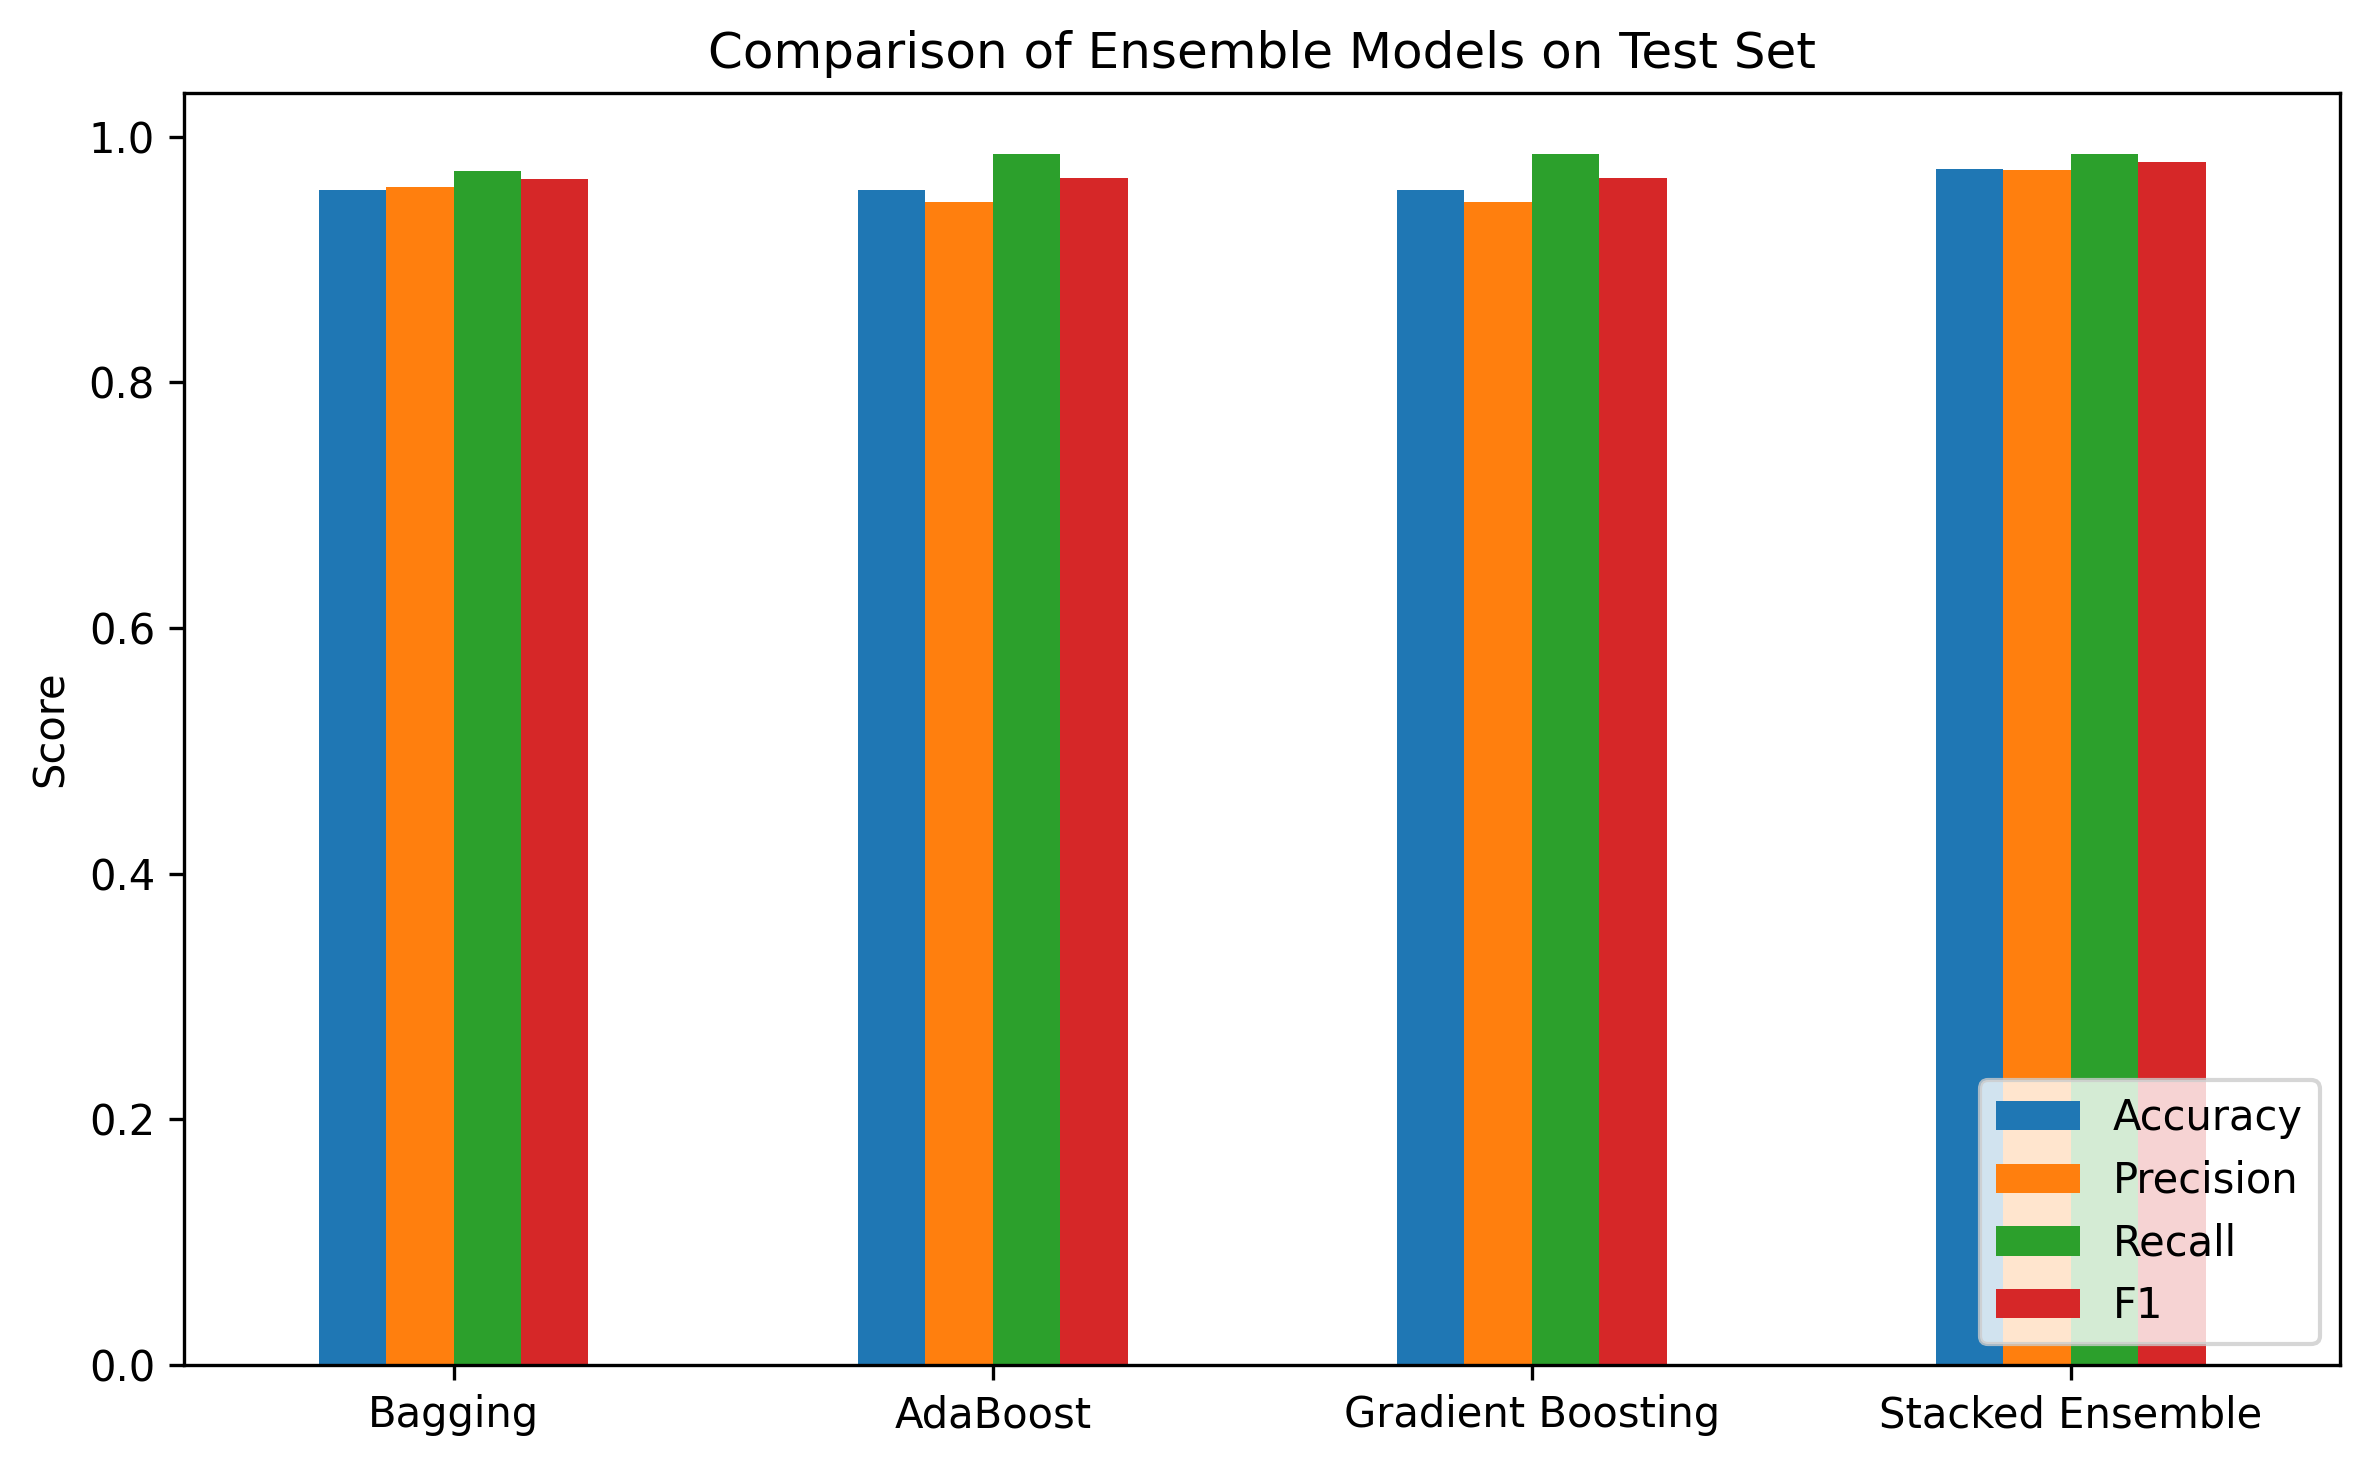
\includegraphics[width=0.7\linewidth]{ensemble_comparison.png}
\caption{Test Set Metrics Comparison Across Ensemble Models}
\end{figure}
\textbf{Inference:} The Stacked Ensemble achieved the highest overall score balance across Accuracy (97.37\%), Precision (0.9726), Recall (0.9861), and F1 Score (0.9793).

\section{5-Fold Cross-Validation Performance Comparison}
\begin{longtable}{|p{3cm}|p{1.5cm}|p{1.5cm}|p{1.5cm}|p{1.5cm}|p{1.5cm}|p{1.8cm}|}
\hline
\textbf{Model} & \textbf{Fold 1} & \textbf{Fold 2} & \textbf{Fold 3} & \textbf{Fold 4} & \textbf{Fold 5} & \textbf{Average} \\ \hline
\endhead
Bagging & 0.9561 & 0.9298 & 0.9386 & 0.9561 & 0.9735 & 0.9508 \\ \hline
AdaBoost & 0.9912 & 0.9386 & 0.9561 & 0.9737 & 0.9735 & \textbf{0.9666} \\ \hline
Gradient Boosting & 0.9737 & 0.9035 & 0.9561 & 0.9737 & 0.9823 & 0.9579 \\ \hline
Stacked Ensemble & 0.9737 & 0.9211 & 0.9649 & 0.9474 & 0.9646 & 0.9543 \\ \hline
\end{longtable}

\section{Observation Questions}
\begin{enumerate}
\item \textbf{How does Bagging reduce variance?} Bagging constructs multiple independent bootstrap samples from the training set and fits an unconstrained base decision tree on each. By averaging predictions across decorrelated trees, high individual tree variance is smoothed out, preventing model overfitting while keeping base estimator bias unchanged.
\item \textbf{How does Boosting address model bias?} Boosting sequentially trains base models, where each subsequent model focuses on misclassified samples or residuals from prior iterations. By iteratively combining weak learners into a strong ensemble, Boosting effectively shrinks model bias and builds sharp decision boundaries.
\item \textbf{Why does stacking benefit from heterogeneous models?} Heterogeneous base models (e.g., decision trees, probabilistic Na\"ive Bayes, and hyper-plane SVMs) make distinct structural errors due to different inductive biases. A meta-learner learns to leverage the unique strengths of each model, resulting in superior generalization over single-family ensembles.
\item \textbf{Which ensemble method performed best and why?} The Stacked Ensemble achieved the highest overall test accuracy (97.37\%) and F1 score (0.9793). Stacking benefited from combining non-linear tree rules, probabilistic estimates, and margin-based decision boundaries, allowing the meta-learner to resolve ambiguous margin cases efficiently.
\end{enumerate}

\section{Discussion}
Comparative analysis across Bagging, Boosting, and Stacking highlights how ensemble learning effectively addresses the bias-variance trade-off. Bagging provides high stability by decorrelating variance-prone base trees. Boosting algorithms (AdaBoost and Gradient Boosting) aggressively minimize bias, achieving up to 98.02\% CV accuracy. Finally, Stacking leverages model diversity to produce the highest test generalization (97.37\% accuracy).

\section{Conclusion}
In this experiment, Bagging, Boosting, and Stacked Ensemble classifiers were successfully implemented and evaluated on the Wisconsin Diagnostic Breast Cancer dataset. Ensemble methods consistently outperformed individual base models. The Stacked Ensemble model delivered the best overall predictive performance (97.37\% accuracy, 0.9793 F1 score, 0.9861 recall), demonstrating the effectiveness of combining heterogeneous classifiers for medical diagnosis tasks.

\section{References}
\begin{enumerate}[label={[\arabic*]}]
\item Scikit-learn Documentation, ``Ensemble Methods,'' \url{https://scikit-learn.org/stable/modules/ensemble.html}
\item Scikit-learn Documentation, ``Bagging Classifier,'' \url{https://scikit-learn.org/stable/modules/generated/sklearn.ensemble.BaggingClassifier.html}
\item UCI Machine Learning Repository, ``Breast Cancer Wisconsin (Diagnostic) Data Set,'' \url{https://archive.ics.uci.edu}
\end{enumerate}

\end{document}
